\documentclass[10pt]{beamer}
% \usepackage{pst-poker}

% \usepackage{mathspec}
% \setmainfont{Liberation Sans}
% \setmathfont(Digits,Latin,Greek){Liberation Sans}
% \usepackage{beamerthemesplit} // Activate for custom appearance

\title{How random are our shuffles?}
\subtitle{STAT 157 Presentation}
\author{Feng Cheng, Lucy Meng}
%\institute{}
\date{Nov.\ 30\textsuperscript{th}, 2023}
\usecolortheme{seahorse}
% \usetheme{Madrid}

\beamertemplatenavigationsymbolsempty
\setbeamertemplate{footline}[frame number]
\setbeamertemplate{frametitle continuation}{}

\usepackage{sansmathfonts}
\usepackage{amsmath,amssymb,amsthm}
\usepackage{mathtools}
\setlength{\parskip}{.5em}

% \usepackage[pdfusetitle,bookmarksnumbered]{hyperref} %load this at the end
% \usepackage[noabbrev]{cleveref}

\newcommand{\blank}{\,\cdot\,}
\newcommand{\id}{\mathrm{id}}
\newcommand{\la}{\langle}
\newcommand{\ra}{\rangle}
\newcommand{\R}{\mathbf{R}}
\newcommand{\where}{\,|\,}
\newcommand{\inp}[2]{\langle #1, #2 \rangle}
\newcommand{\nm}[1]{\lVert #1 \rVert_\mathrm{TV}}
\newcommand{\tmix}{t_\mathrm{mix}}
\newcommand{\abs}[1]{\lvert #1 \rvert}
\newcommand{\ol}[1]{\overline{#1}}

\renewcommand{\Pr}{\mathbf{P}}
\newcommand{\E}{\mathbf{E}}
\newcommand{\Var}{\operatorname{Var}}

\newcommand{\df}[1]{\textbf{#1}} % definition
\newcommand{\codevar}[1]{\ensuremath{\mathtt{\textcolor{brown}{#1}}}} % variable in code

\newtheorem{prop}[theorem]{Proposition}

\begin{document}

\begin{frame}
    \titlepage
\end{frame}

\begin{frame}{Outline}
    \tableofcontents
\end{frame}

\section{Shuffle models}
\subsection{Top-to-random shuffle}
\begin{frame}[allowframebreaks]{Top-to-random shuffle}
    \begin{itemize}
        % assign mu to each group element h
        \item For a random walk on a finite group $G$, the transition matrix $P$ follows
        \[P(g,hg) = \mu(h).\]
        The random walk has a stationary distribution $\pi$ uniform over $G$.
        \item Our top-to-random shuffle is a random walk on $G = S_n$, the group of permutations on $n$ elements. Mathematically \[
        \mu(\sigma) = \begin{cases}
            \frac{1}{n} & \text{if }\sigma = (k\ \cdots\ 2\ 1) \text{ for }1 \leq k\leq n; \\
            0 & \text{otherwise}.
        \end{cases}
        \]
        \item Shuffle chains
        % every permutation generated by mu(sigma) > 0
        are \emph{irreducible}, so the uniform measure over $S_n$ is the unique stationary distribution.
        \item Since $\mu(\id) > 0$, the chain is also \emph{aperiodic}.
        % aperiodicity and irreducibility allows us to discuss the distance
    \end{itemize}    
    \framebreak
        How to quantify the randomness of our shuffle?
    \begin{itemize}
        \item Recall $\nm{\mu - \nu} = \max_{A \subseteq S_n}\abs{\mu(A) - \nu(A)}$.
        \item Also recall \[
            d(t) = \max_{\sigma \in S_n} \nm{P^t(\sigma,\blank) - \pi} = \nm{P^t(\id,\blank) - \pi},
        \] and \[\tmix(\epsilon) = \min\{t:d(t) \leq \epsilon\}.\]
        We want $t$ such that \[\nm{P^t(\id,\blank) - \pi} \leq \epsilon.\]
    \end{itemize}
\end{frame}

\begin{frame}[label=mainthm]{Main theorem of top-to-random shuffle}
    \begin{theorem}[Aldous-Diaconis 1986]
    For $\alpha \geq 0$, we have 
        \begin{enumerate}[(i)]
            \item $d(n\log n+ \alpha n) \leq e^{-\alpha}$;
            \item % For any $\epsilon > 0$, there exists $K$ such that given $c > K$, for all sufficiently large $n$, $d(n\log n - cn) \geq 1 - \epsilon$.
            $\liminf_{n\to\infty} d(n\log n - \alpha n) \geq 1 - 2 e^{2-\alpha}$.
        \end{enumerate}
    \end{theorem}
    % describe the behavior of d around n log n
    We need about $52\log(52) \approx 206$ top-to-random shuffles to mix the cards!
\end{frame}

\subsection{Riffle shuffle}
\begin{frame}[allowframebreaks]{Riffle shuffle}
        How to model the random cut into the two decks? How to riffle the two decks together?
        \begin{enumerate}[a)]
            \item $M \sim \operatorname{Binomial}(n,1/2)$ cards in the left deck and $n - M$ in the right. Then $\binom{n}{M}$ ways to riffle together.
            \item Still $M \sim \operatorname{Binomial}(n,1/2)$.
            
            At time $t$ the left deck has $a$ remaining cards and the right deck has $b$ remaining, drop the left (resp.\ right) bottom card with probability $\frac{a}{a+b}$ (resp.\ $\frac{b}{a+b}$).
        \end{enumerate}
        It is very easy to see that the two are the same with: 
        \[\mu(\sigma) = \begin{cases}
            (n+1)/{2^n} & \text{if }\sigma = \mathrm{id}; \\ % n+1 comes from M = 0 to n
            1/2^n & \text{if }\sigma\text{ has exactly two rising sequences}; \\
            0 & \text{otherwise}.
        \end{cases}\]
        This is called the \df{Gilbert-Shannon-Reeds (GSR) model}.

    \framebreak
    % Suffices to consider the reverse distribution $\widehat{Q}$ given by $\widehat{Q}(\sigma) = Q(\sigma^{-1})$, as $\nm{Q^t - \pi} = \nm{\widehat{Q}^t - \pi}$.
    % This inverse shuffle can be characterized by 
    Other characterizations: inverse description, sequential description
    \begin{theorem}[Bayer-Diaconis 1992]
        \[
        \nm{Q^k - \pi} = \frac{1}{2}\sum_{j=0}^{n-1} A(n,j)\bigg\lvert \binom{n+2^k-j-1}{2^{kn}} - \frac{1}{n!}\bigg\rvert,
        \]
        where A(n,j) is the number of permutations on n symbols with j descents. % computed easily via recursion
    \end{theorem}
\end{frame}
\begin{frame}[label=BD1992fig]{``Seven-shuffle"}
    \begin{figure}
        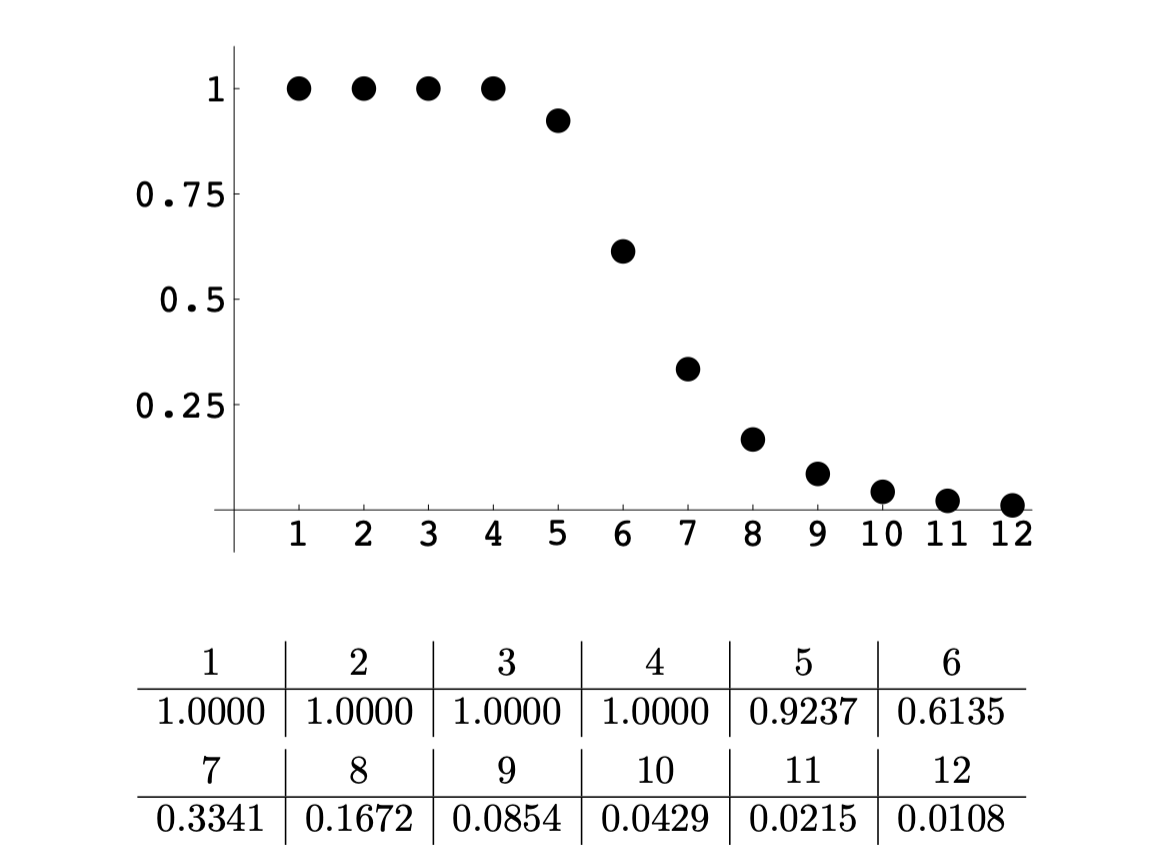
\includegraphics[width = 0.8\textwidth]{convfig.png}
        \caption{$n = 52, 1\leq k \leq 12$}
    \end{figure}
\end{frame}

\section{Analysis of the top-to-random shuffle}

\begin{frame}{Main theorem of top-to-random shuffle}
    \begin{theorem}[Aldous-Diaconis 1986]
    For $\alpha \geq 0$, we have 
        \begin{enumerate}[(i)]
            \item $d(n\log n+ \alpha n) \leq e^{-\alpha}$;
            \item % For any $\epsilon > 0$, there exists $K$ such that given $c > K$, for all sufficiently large $n$, $d(n\log n - cn) \geq 1 - \epsilon$.
            $\liminf_{n\to\infty} d(n\log n - \alpha n) \geq 1 - 2 e^{2-\alpha}$.
        \end{enumerate}
    \end{theorem}
    We will prove (i). See MCMT \S 7.4.1 for a proof of (ii).

    Recall $\E(\tau_\mathrm{coupon}) = n \sum_{k=1}^n\frac{1}{k} \approx n\log n$.
\end{frame}

\subsection{Connection to the coupon collector's problem}
\begin{frame}{Observation}
    Say the original bottom card is $\spadesuit$\!\! K. We claim that one shuffle after the first time $\spadesuit$\!\! K reaches the top, the cards are completely mixed.

    We call this $\tau_\mathrm{top}$.

    Let $\tau_\mathrm{coupon}$ be the total number of coupons collected when the set first contains all $n$ types of coupons.

    We claim $\tau_\mathrm{coupon} = \tau_\mathrm{top}$. % reverse coupon collector; in coupon collector difficulty increases, in top diffculty decreases
\end{frame}

\begin{frame}{Connection to the coupon collector's problem}
    \begin{prop}[2.4 MCMT]
        For any $\alpha > 0$, \[\Pr\bigl(\tau_\mathrm{coupon} > \lceil n\log n + \alpha n\rceil\bigr) \leq e^{-\alpha}.\]
    \end{prop}
\end{frame}

\subsection{Intro to strong stationary times}

\begin{frame}{Stationary times}
    \begin{itemize}
        \item We call $\tau$ is a \df{stationary time}\footnote{measure-theoretic setup omitted} if for all state $y$ \[\Pr_x(X_\tau = y) = \pi(y).\]
        \item We call $\tau$ is a \df{strong stationary time}\footnotemark[\value{footnote}] if for all time $t$ and state $y$ \[\Pr_x(\tau = t, X_\tau = y) = \Pr_x(\tau  = t)\pi(y),\] i.e., $X_\tau$ has distribution $\pi$, and is independent of ${\tau = t}$.
        % sum the t's we see X_t = pi in dist., independence is then clear
        \item Our $\tau_\mathrm{top}$ is a strong stationary time for the top-to-random shuffle chain. % Whenever tau is, X_t has distribution pi.
    \end{itemize}
    
    
\end{frame}

\begin{frame}{Sketch proof of the main theorem (upper bound)}
    \begin{theorem}[6.11 MCMT]
        If $\tau$ is a strong stationary time for the starting state $x$, then \[
            \nm{P^t(x,\blank) - \pi} \leq \Pr_x(\tau > t).
        \]
        % time reaching stationary
    \end{theorem}
    \begin{prop}[2.4 MCMT]
        Let $\tau$ be the total number of coupons collected when the set first contains all $n$ types of coupons, then for any $\alpha > 0$, \[\Pr\bigl(\tau > \lceil n\log n + \alpha n\rceil\bigr) \leq e^{-\alpha}.\]
    \end{prop}
\end{frame}

\subsection{The cutoff phenomenon}
\begin{frame}{Cutoff phenomenon (with a window)}
    \begin{figure}
        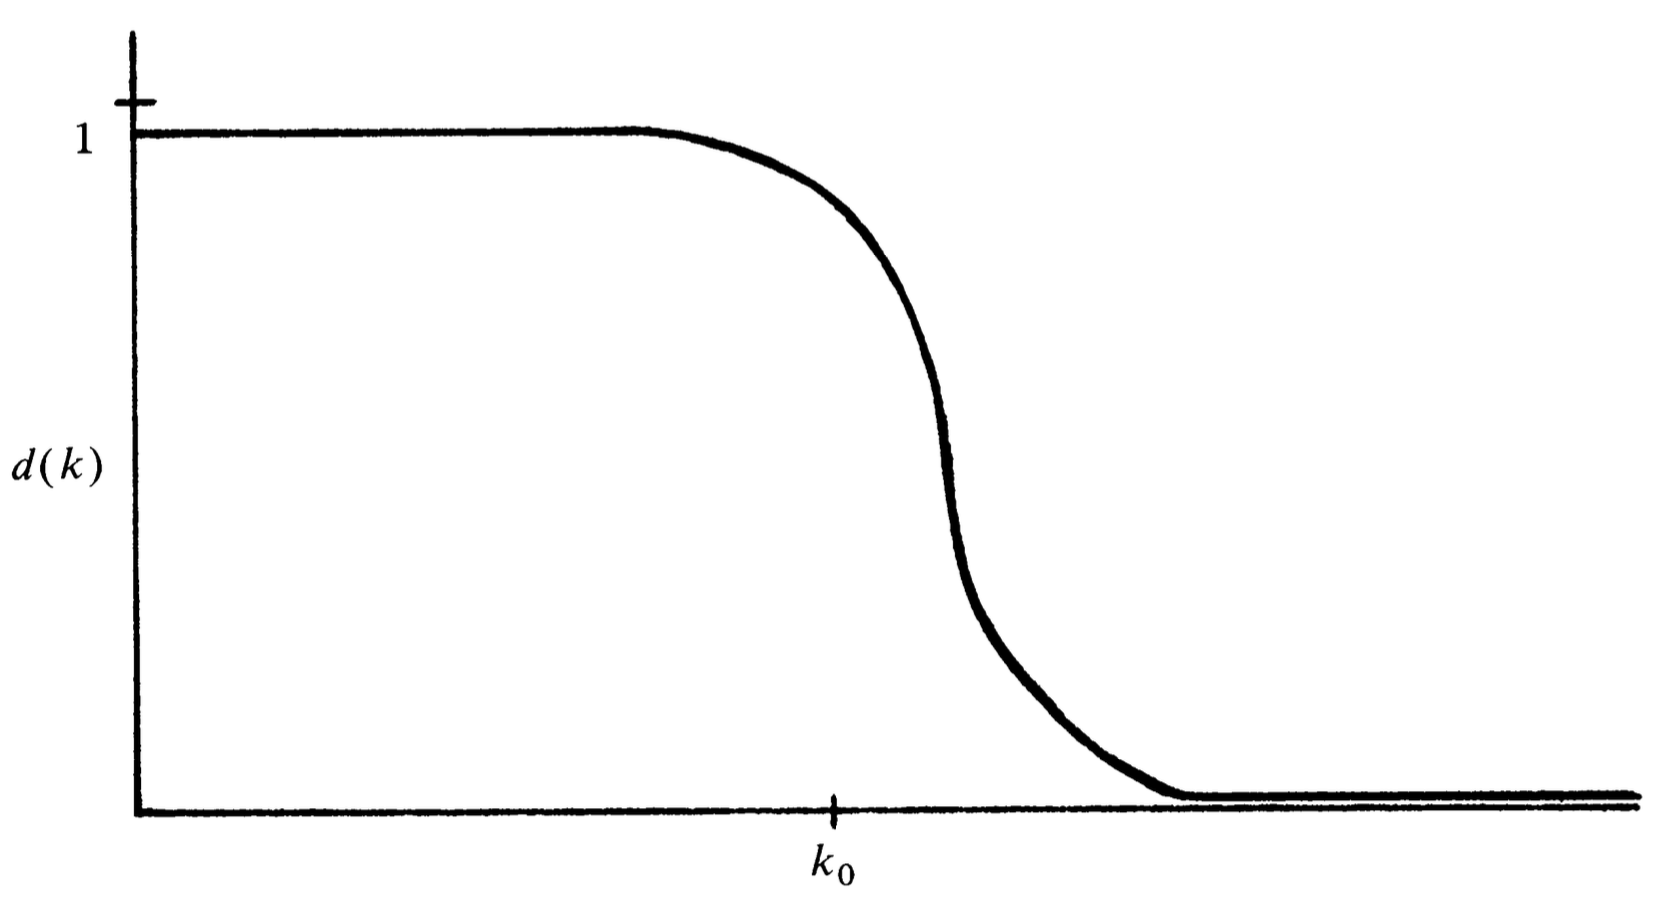
\includegraphics[width = 0.7\textwidth]{cutoff.png}
    \end{figure}
    There is a critical $\tmix^{(n)} = k_0$ such that $d(k_0 + o(k_0)) \approx 0$ and $d(k_0 - o(k_0)) \approx 1$. Asymptotically as $n\to \infty$ we should see the plot becoming a step function at $k_0$.
\end{frame}

\begin{frame}{Main theorem of top-to-random shuffle}
    \begin{theorem}[Aldous-Diaconis 1986]
    For $\alpha \geq 0$, we have 
        \begin{enumerate}[(i)]
            \item $d(n\log n+ \alpha n) \leq e^{-\alpha}$;
            \item % For any $\epsilon > 0$, there exists $K$ such that given $c > K$, for all sufficiently large $n$, $d(n\log n - cn) \geq 1 - \epsilon$.
            $\liminf_{n\to\infty} d(n\log n - \alpha n) \geq 1 - 2 e^{2-\alpha}$.
        \end{enumerate}
    \end{theorem}
    What happens when $\alpha \to \infty$? What about $-\infty$? % exponentially going to 1 and 0 resp.
\end{frame}

\againframe<2>{BD1992fig}

\begin{frame}{Asymptotic result of the riffle shuffle}
    \begin{theorem}[Bayer-Diaconis 1992]
        If $n$ cards are riffle shuffled $k = \frac{3}{2}\log_2(n) + c$ times, then for large $n$, \[
            \nm{Q^k - \pi} = 1 - 2\Phi\Bigl(\frac{-2^{-c}}{4\sqrt{3}}\Bigr) + O(n^{-1/4}).
        \]
    \end{theorem}
    \begin{itemize}
        \item $\tmix^{(n)} = \frac{3}{2}\log_2(n)$ asymptotically.
        \item As $c \to -\infty$, $\nm{\blank} \to 1$ doubly exponentially fast.
        \item As $c \to \infty$, $\nm{\blank} \to 0$ exponentially fast.
    \end{itemize}
\end{frame}

\begin{frame}{Summary}
    \begin{itemize}
        \item Cutoff phenomenon prevalent in card shuffling
        \item Strong stationary time as an important technique
        \item Applications in cryptography
        \item More shuffles (random transposition, Hindu, Thorp, L-reversal, etc.)
    \end{itemize}
\end{frame}

\section{References and recommendations for further reading}
\begin{frame}{Sources}
\begin{itemize}
    \item \textit{Markov Chain and Mixing Time} by Levin, Peres, and Wilmer
    \item ``Shuffling cards and stopping models'' (1986) by Aldous and Diaconis
    \item ``Trailing the dovetail shuffle to its lair'' (1992) by Bayer and Diaconis
    \item ``Analysis of top to random shuffles'' (1992) by Diaconis, Fill, and Pitman
    \item \textit{The Mathematics of Shuffling Cards} by Diaconis and Fulman
\end{itemize}

Check out Diaconis Numberphile videos as well!
\end{frame}
% \section[Outline]{}
% \frame{\tableofcontents}

% \section{Different Shuffles}
% % \subsection{Top-to-random shuffle}
% \frame
% {
%   \frametitle{Features of the Beamer Class}

%   \begin{itemize}
%   \item<1-> Normal LaTeX class.
%   \item<2-> Easy overlays.
%   \item<3-> No external programs needed.
%   \end{itemize}
% }

% \subsection{Detail of the Beamer Class}
% \frame{
% 	\frametitle{List}
	
% 	\begin{enumerate}[i)]
% 	\item This is good.
% 	\item This is bad.
% 	\item This is neither good nor bad.
% 	\end{enumerate}
% 	\begin{theorem}
% 	This is a theorem.
% 	\end{theorem}
% 	\begin{definition}
% 	This is a definition.
% 	\end{definition}
% 	\begin{proof}
% 	This is a proof.
% 	\end{proof}
% }

% \section{Blocks}
% \frame{
% 	\begin{block}{Sample}
% 		\blindtext
% 	\end{block}
	
% }

\end{document}
